\chapter{Fundamental Mathematics and Notation}
\label{chap:fundamentals} 
It is necessary to recall some fundamental mathematical concept to understand the subsequent chapters and introduce the notations used in the thesis.
This chapter introduces the essential mathematical backgrounds that are directly relevant to the contents of this thesis to help readers a clear understanding of the subsequent chapters.
The theoretical discussion will often appear with minimal definition and citation of the details works since details discussion is beyond the scope of this thesis.
We refer to \cite{lidl_niederreiter_1996, book_HFFMullen2013, book_CMSSmart2015, book_GPCMrabet2016, book_CSCBlahut} for more details of the topics. 
As an additional purpose, this chapter specifies most of the notations that will appear in the upcoming chapters.

Cryptography deals with numbers mostly integers.
It is essential to have a good understanding of the underlying mathematical concepts to understand modern cryptography.
The following concepts are the basis for the discussion of the subsequent chapters.

\section{Modular Arithmetic}
\label{sec:chap:fund:modular_arithm} 
Modular arithmetic is the fundamental tool for modern cryptography especially public key cryptosystems.
\begin{definition}[Modular Arithmetic\index{modulus}]
	Let  $p$ be a positive integer named as the modulus \index{modulus} and  $a$ and $b$  are two arbitrary integers. 
	If  $p$ divides $b-a$  then we can write
	$$ a \equiv b ~(\bmod ~p)$$
	and express as $a$ and $b$ are congruent modulo $p$.
\end{definition}
\begin{example}
	Let, $p =7$, $a=19$ and $b=5$ then 
	$19  \equiv  5 ~(\bmod ~7) $.
\end{example}

\begin{example}
	Let, $p =7$, $a=-17$  and $b=11$. Then $-17  ~(\bmod ~7)  = 4$ and $11 ~(\bmod ~7) = 4$. 
	We can write 
	$$-17  \equiv  11 ~(\bmod ~7) $$ 
	and usually express $-17$ and $11$ are congruent modulo $7$.
\end{example}

\section{Group, Ring, Field}
\label{sec:chap:fund:group}
\subsection{Group}
The concept of group \index{group} is very fundamental to understanding cryptography. It is an algebraic system defined as follows.
\begin{definition}[Group\index{group}]
	A group \index{group} is a non-empty set $\mathbb{G}$ with a binary operation $\circ$ on its elements denoted as  $\langle\mathbb{G}\index{group},\circ\rangle$,  sometimes denoted by   $\mathbb{G}$ only, which satisfies the following axioms.
	\begin{quote}
		\begin{description}
			\item[Closure] The group is closed under the operation $\circ$, i.e.  $\forall a \in\mathbb{G}$, and $\forall b \in\mathbb{G}$ the result of $ (a\circ b) = c \in \mathbb{G}$. \footnote{$\forall$ symbol bears is usual notation \textit{"for all"} }
			
			\item[Identity element] There exist an \textbf{identity element \index{Identity element}} $e$ also know as \textit{neutral element} or \textit{unit element} in $\mathbb{G}$ such that $\forall a \in\mathbb{G} \index{group}$,  $a\circ e = e\circ a = a$.
			
			\item[Inverse element] For ${\forall}a \in\mathbb{G}\index{group}$, there exists an element $b\in\mathbb{G}\index{group}$ such that $a\circ b=e=b\circ a$, where $b$ is called inverse element of $a$.
			
			\item[Associativity] Elements in  group $\mathbb{G}$ should follow associativity. i.e. $(a\circ b)\circ c=a\circ (b\circ c)$ for all $ a,b,c\in\mathbb{G}\index{group}$.
			
		\end{description}
	\end{quote}
\end{definition}

\begin{definition}[Commutative Group\index{group}] \hspace{0em}
	\begin{quote}\begin{description}
			A group \index{group} $\mathbb{G}\index{group}$ will be commutative if $a\circ b=b\circ a$ for all $a,b \in\mathbb{G}\index{group}$.
	\end{description}\end{quote}
	\qed
\end{definition}
A commutative group is also called \textit{abelian} group.

\begin{example} \label{example_group}
	The set of integers $\mathbb{Z}$ forms a group under the group operation of addition $+$ denoted as $(\mathbb{Z},+)$. $0$ is the identity element of the group.
\end{example}
\begin{example}\label{example_notgroup}
	The set of positive integers $\mathbb{N}$ under addition does not form a group since elements have not inverse.
\end{example}
%For example, the algebraic system $\langle\mathbb{Z},+\rangle$ is an infinite commutative group\index{group}, where $\mathbb Z$ is the integer set, and $+$ means the ordinary addition for integers. For a finite group\index{group}, its order\index{group order} is defined as follows.
\begin{definition}[Order of a Group\index{group}]\hspace{0em}
	The order of a group $\mathbb{G}$ \index{group order} often denoted as $\#\mathbb{G}\index{group}$ is the number of elements in the group\index{group} $\mathbb{G}\index{group}$.
	\qed
\end{definition}

\begin{remark}
	Groups order can be finite and infinite. In example \ref{example_group}, $(\mathbb{Z},+)$ has infinite order.
\end{remark}

\begin{definition}[Order of group element\index{order of element}]
	For an element $a\in\mathbb{G}\index{group}$, the smallest positive integer $m$ such that $a^{m}=e$ is called the order\index{order} of $a$, where $e$ is the identity element in $\mathbb{G}\index{group}$.
	\qed
\end{definition}

\begin{example}{Finite group:  \index{finite group} } \label{definition_finite_group}
	As shown in example \ref{example_notgroup}, the set $\mathbb{N}$ under addition does not form a group since it does not satisfy the group\index{group} axioms. 
	Let us consider a set $\mathbb{N}_{n}$ under the operation $\mod n$  such that 
	$$ \mathbb{N}_{n} = \{0,1,2,3, \cdots, n-1\}$$
	where $n \in \mathbb{N}$.
	It means $\mathbb{N}_{n}$ is the set of remainders under ``$\bmod\ n$''.
	Recall the modular arithmetic that 
	$$a+b\equiv c\ \ \bmod n\hspace{3em}a,b\in \mathbb{N}_{n},\label{Sum Definition}$$
	means $c$ is  associated to a remainder on division by $n$ when $a+b=c\notin\mathbb{N}_{n}$. 
	It makes $c$ belongs to $\mathbb{N}_{n}$ making $( \mathbb{N}_{n},+)$ forming a group\index{group}.
	In also includes element $0$ which acts as an identity element.
\end{example}

\begin{definition}[Group generator\index{group}]
	For a given group\index{group} $\mathbb{G}\index{group}$ if there is an element $g\in\mathbb{G}\index{group}$ such that for any $a\in\mathbb{G}\index{group}$ there exist an unique integer $i$ with $a=g^{i}$ then $g$ will be called a   generator\index{generator} of  $\mathbb{G}\index{group}$
	\qed
\end{definition}

\begin{definition}[Cyclic Group\index{group}]
	A group\index{group} $\mathbb{G}\index{group}$ will be {\em cyclic} if there exist at least one generator $g \in \mathbb{G}$. Cyclic group usually expressed as $\mathbb{G} = \langle g \rangle$
	\qed 
\end{definition}

\begin{remark}
	The number of generator in a group $\mathbb{G}\index{group}$ of order $n$ is defined by Euler's totient function $\phi(n)$\footnote{When $n$ is a positive integer, Euler's totient function $\phi(n)=$ number of positive integers less than or equal to $n$ that are co-prime to $n$}.
	If $n$ is a prime $p$ then the  group $\mathbb{G}$ will be called prime order group and it will have $\phi(p) = p-1$ generators.
\end{remark}

\begin{definition}[Cyclic Group\index{group}]
	A group\index{group} $\mathbb{G}\index{group}$ will be {\em cyclic} if there exist at least one generator $g \in \mathbb{G}$. Cyclic group usually expressed as $\mathbb{G} = \langle g \rangle$ 
	\qed 
\end{definition}

In this case, we use the notation $\langle\mathbb{G}\index{group},\circ\rangle$; there exists some ambiguity which operation we consider.
Therefore, the following two types of group nations are prevalent in literature.

\begin{definition}[Additive group\index{additive group}]
	A cyclic group is called \textit{additive} if we tend to write its group operation in the same way we do additions, that is 
	$$f = g + x$$ 
	can also appear as $[x]g$ meaning applying $x -1$ times addition operator $+$ on $g$.
	It is also common to write as $x \cdot g$.
	For example, $1$ is one of generators in group $(\mathbb{Z}_5, + )$ under addition modular $5$, then $1 \cdot 4$ can be written as $$ 4 = 1+ 1+ 1+1.$$
	\qed
\end{definition}

\begin{definition}[Multiplicative group\index{multiplicative group}]
	A cyclic group is called \textit{multiplicative} if we tend to write its group operation in the same way we do multiplication, that is 
	$$f =  g \cdot x ~\text{or}~ f = g^x$$ 
	\qed
\end{definition}

\begin{remark}
	In both notation the $x$  is an integer called the \textit{discrete logarithm} of $h$ to the base $g$.
\end{remark}
\begin{remark}
	Unless otherwise stated, through out this thesis we will use the $xg$ notation for ordinary addition e.g. $a+a=2a$ and $a+a+a=3a$ and for multiplicative notation, these will denoted by $a^2$, $a^3$.
\end{remark}

From the definition cyclic group, it can be see visualized that any elements in cyclic a group\index{cyclic group} are generated with iterative operations of generator\index{generator} $g$. 
\fgref{Cyclic group} shows this schematically.
\begin{figure}[ht]
	\begin{center}
		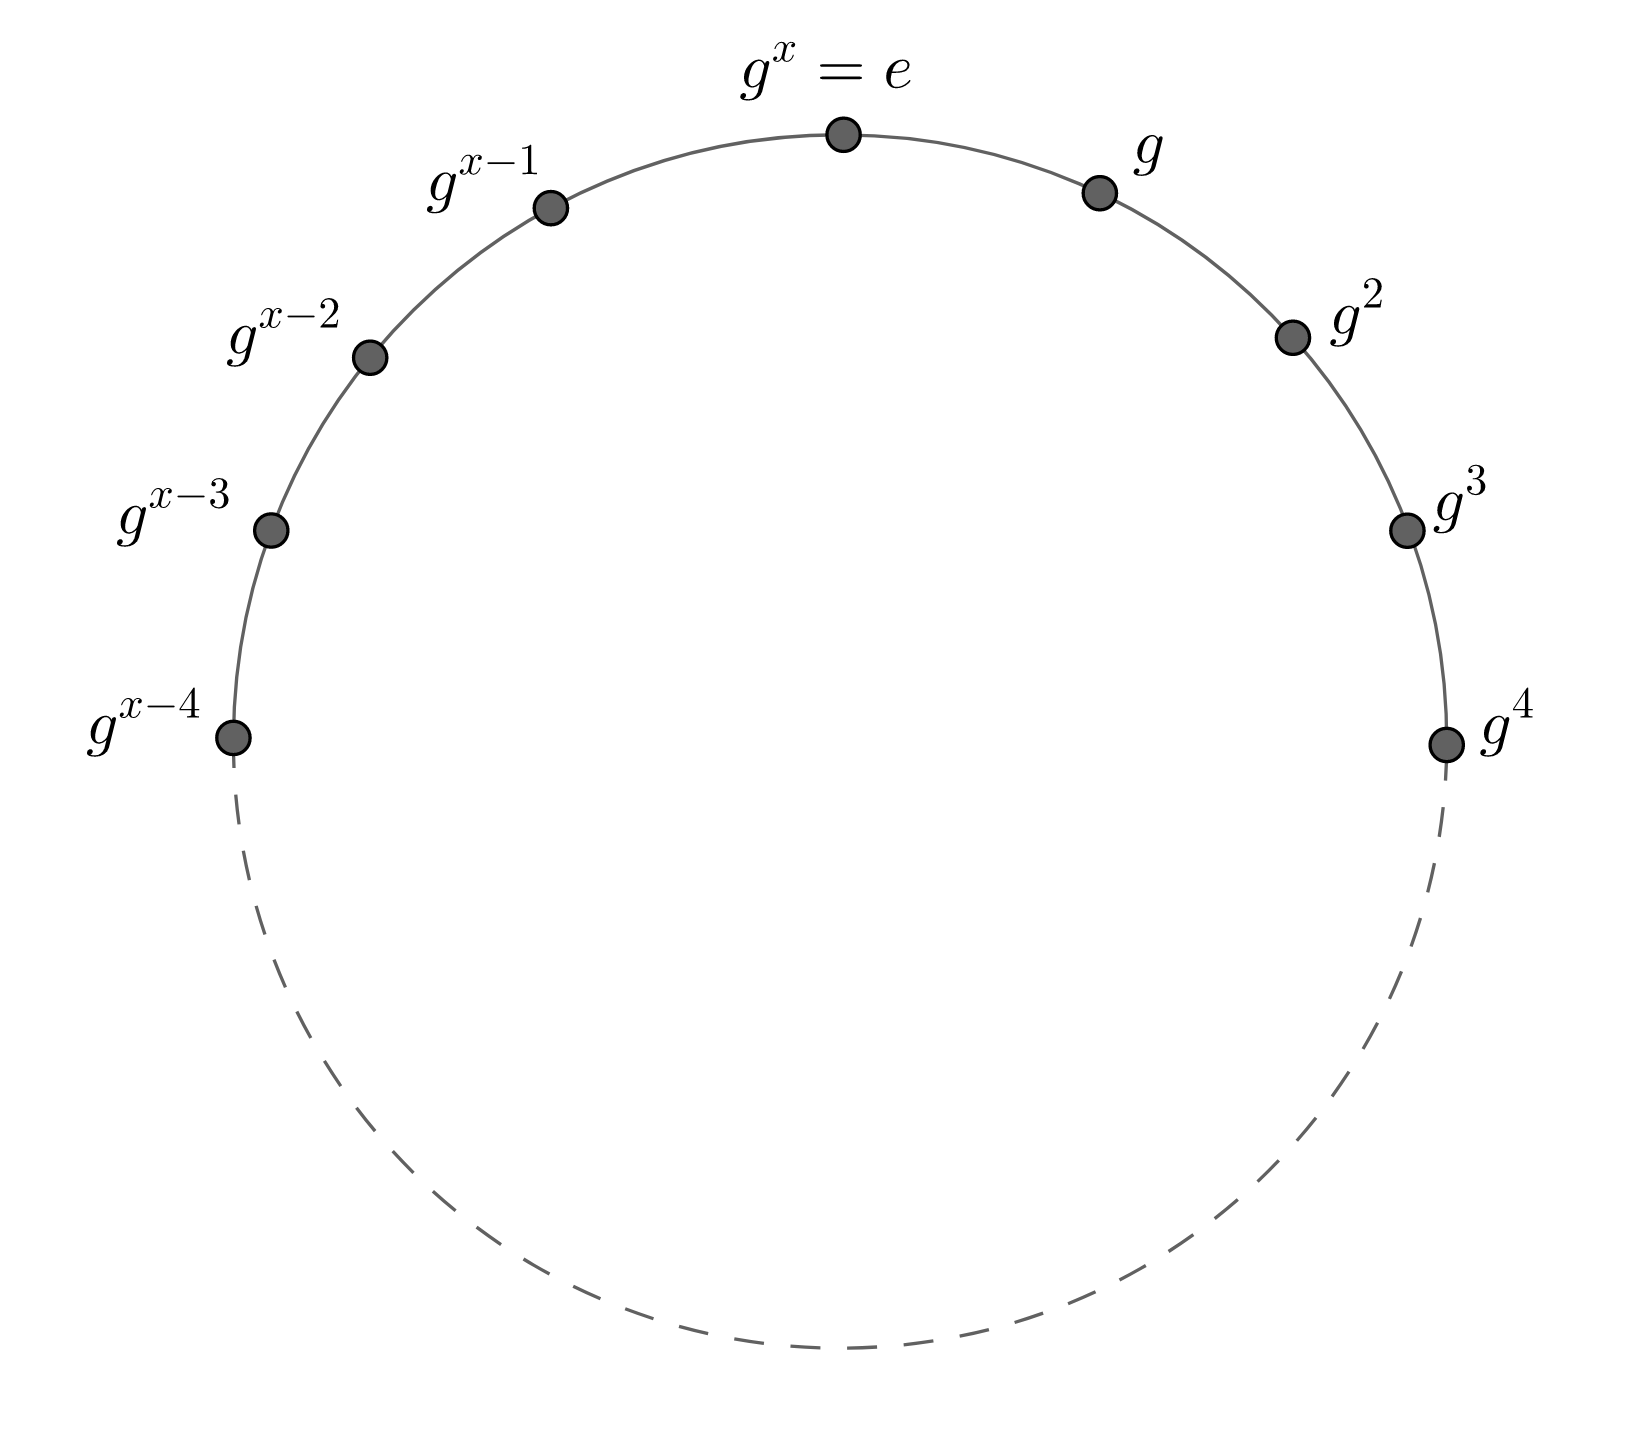
\includegraphics[width=.6\linewidth, height=.67\textheight, keepaspectratio]{Figures/cyclicgroup}
		\caption{Cyclic group\index{cyclic group}\index{group}.}
		\label{Cyclic group}
	\end{center}
\end{figure}

A a well known practice of presenting a finite group's\index{group} operation is {\em Cayley table\index{Cayley table}} as shown in example \ref{example_Cayleytable}.
Cayley table\index{Cayley table} shows all possible group operation that can be performed in a finite group.

\begin{example} \label{example_Cayleytable}
	The Cayley table\index{Cayley!Cayley table} for the group\index{group} $\mathbb{Z}_4$ is:
	\begin{center}
		\begin{tabular}{c|cccc}
			$\oplus_4$&\em 0&\em 1&\em 2&\em 3       \\
			\hline
			\em 0&\em 0&\em 1&\em 2&\em 3       \\
			\em 1&\em 1&\em 2&\em 3&\em 0       \\
			\em 2&\em 2&\em 3&\em 0&\em 1       \\
			\em 3&\em 3&\em 0&\em 1&\em 2       \\
		\end{tabular}
	\end{center}
\end{example}
In the above example of group $(\mathbb{Z}_4,+)$, there are $\phi(4)=2$ generators, $3$ and $1$.

\begin{definition}[Subgroup\index{subgroup}]
	Let $\mathbb{H}$ be  a non-empty subset  fo group $\mathbb{G}$, $\mathbb{H}$  will be called subgroup of $\mathbb{G}$ if  $\mathbb{H}$  itself follows group axioms and $\mathbb{H}$ has the same identity element of group $\mathbb{G}$. 
	\qed
\end{definition}

\begin{theorem}[Lagrange's Theorem:]
	Let $\mathbb{G}$ be a finite abelian group and $\mathbb{H}$ is a subgroup of $\mathbb{G}$.  The order of $\mathbb{G}$, $\#\mathbb{G}$ is divisible by the order of subgroup $\mathbb{H}$, $\#\mathbb{H}$ i.e.   $\#\mathbb{H} | \#\mathbb{G}$.
	\qed
\end{theorem}

\begin{theorem}[Fermat’s Little Theorem:]
	Let $p$ is a prime and $a \in \mathbb{Z}$, then $$a^p = a ~(\bmod ~p)$$
	\qed
\end{theorem}
Fermat’s \textit{little theorem} is a special case of Lagrange’s theorem.


\subsection{Homomorphism in Groups \index{homomorphism}}
Morphisms in groups have often used the research of cryptography and inseparable to for pairing-based cryptography research.
\begin{definition}[Homomorphism\index{rings}]
	Let $(\mathbb{G},\circ)$ and $(\mathbb{G}^{'},\star)$ be two groups with identity elements $e$ and $e'$ respectively.
	A homomorphism  is a map $f$ which preserves the group structure while the elements are mapped from $(\mathbb{G},\circ)$ to $(\mathbb{G}^{'},\star)$.
	\qed
\end{definition}
A homomorphic map obeys the following conditions:
\begin{itemize}
	\item $\forall a,b \in \mathbb{G}$, $f(a \circ b) = f(a) \star f(b)$.
	\item  For every $a \in \mathbb{G}$, the inverse map is $f(a^{-1}) = f(a)^{-1}$.
	\item  Identity element mapping also preserves the structure i.e. $f(e) =e'$.
\end{itemize}

\subsubsection{Types of Homomorphism}
\begin{quote}
	\begin{description}
		\item[Isomorphism \index{Isomorphism}] If an element from $\mathbb{G}$  and $\mathbb{G}^{'}$ have bijective relation then $\mathbb{G}$ and $\mathbb{G}^{'}$ are isomorphic to each other.
		
		\item[Endomorphism  \index{Endomorphism}]  If elements from the group $(\mathbb{G},\circ)$ are mapped to itself, then it is called endomorphism. 
		A frequently used endomorphism in cryptographic algorithms is Frobenius endomorphism. 
		
		\item[Authomorphism  \index{Authomorphism}] If an element of a group has both endomorphism and isomorphism then it is called automorphism.
	\end{description}
\end{quote}

\begin{definition}[Kernel\index{kernel}]
	Let $(\mathbb{G},\circ)$ and $(\mathbb{G}^{'},\star)$ be two groups with identity elements $e$ and $e'$ respectively and $f$ is homomorphism from $(\mathbb{G},\circ)$ to $(\mathbb{G}^{'},\star)$.
	The kernel of $f$ is denoted as $\text{Ker}\{f\}$, defined by 
	$$\text{Ker}(f) = \{ a \in \mathbb{G}: f(a) = e'\}$$.
	\qed
\end{definition}

%--------------------------------------
%--------------------------------------
\subsection{Ring}
The concept of \textit{Ring} will not come as frequently as group and field in the subsequent chapters. 
However, it is relevant to define the ring to understand the related concept.
\begin{definition}[Ring \index{ring}]
	A \textbf{ring} $\mathbb{R}$ is an algebraic structure with two operations, i.e. addition  $+$ and  multiplication $\cdot$  usually denote as $\mathbb{R},+,\cdot$.
	\begin{itemize}
		\item $\mathbb{R}$ is abelian group under addition operation.
		\item Under multiplication, $\mathbb{R}$ is closed and associative with identity element is $1$.
		\item  Multiplication is distributive over addition: $ \forall a, b, c \in \mathbb{R}: a\cdot (b+c) = a\cdot b + a\cdot c$.
	\end{itemize}
	\qed
\end{definition}
If multiplication operation is commutative, $\mathbb{R}$  forms a commutative ring.
%\begin{example}
%    TODO
%\end{example}
\begin{definition}[Multiplicative Inverse Modulo $n$ \index{multiplicative inverse}]
	Let $\mathbb{Z}_n$ be a set under modulo $n$ and $a \in \mathbb{Z}_n$. 
	The multiplicative inverse modulo $n$ of $a$ can be written as  follows:
	$$a\cdot x \equiv  1 \bmod n.$$
	The value $x$ is the multiplicative inverse modulo $n$ of $a$, often written as $a^{-1}$.
	\qed
\end{definition}
Such value of $x$ only exists if $\text{gcd}(x,n)=1$.
If $n=p$ is a prime, then every non-zero element in the set $\mathbb{Z}_p$ will have a multiplicative inverse.
Such $(\mathbb{Z}_p,+,\cdot)$ will be a ring and having the above property it will form a field.

\subsection{Field}
\begin{definition}[Field]
	A field $(\f{},+,\cdot)$ is a set that obeys two binary operations denoted by $+$ and $\cdot$, such that:
	\begin{itemize}
		%        \begin{itemize}
		\item $\f{}$ is a commutative group concerning $+$ having identity element $0$.
		
		\item Let ${\f{\,}}^{\ast}\!\!$ is a subset of $\f{}$ having only not-zero element of $\f{}$ i.e. ${\f{}}^{\ast}  = {\f{} ~\backslash \{0\}}$. 
		Then ${\f{\,}}^{\ast}\!\!$ will be called a commutative group respect to multiplication$\cdot$  where every element should have multiplicative inverse in  ${\f{\,}}^{\ast}\!\!$.
		\item For all $a,b,c \in\f{}$  the distributive law will be followed, e.g. $a\cdot(b+c)=a\cdot b+a\cdot c$ and $(b+c)\cdot a=b\cdot a +c\cdot a$.
	\end{itemize}
	%\end{itemize}
	\qed
\end{definition}
%In general, the elements $0$ and $1$ denote the unit elements regarding to addition $+$ and multiplication $\cdot$, respectively.
\begin{definition}[Subfield \index{subfield}]\hspace{0em} \label{definition_subfielf}
	Let $\f{1}$ is a subset of field $\f{}$. $\f{1}$ will be called a subfeld if $\f{1}$ itself obeys the laws of field with respect to the field operation inherited from  $\f{}$.
	\qed
\end{definition}
\begin{remark}
	In Definition \ref{definition_subfielf}, $\f{}$ is called an {\em extension field} of $\f{1}$.
	If $\f{1}\neq \f{}$, then $\f{1}$ is a {\em proper subfield} of $\f{}$.
\end{remark}

\begin{definition}[Order of Finite Field \index{order of field}]\hspace{0em}
	The order is the number of elements in $\f{}$. If the order of $\f{}$ is finite, $\f{}$ is called finite field. 
	\qed
\end{definition}
\begin{definition}[Characteristic of Finite Field \index{field characteristics}]\hspace{0em}
	Let $\f{}$ be a field and smallest positive number $n$ such that $n \cdot a= 0$ for every $a\in \f{}$. Such $n$ is called characteristic. If there is no such $n$ in  $\f{}$ then $\f{}$ has characteristics $0$.
	\qed
\end{definition}

Most of the works presented in this dissertation deal with finite fields only. 
A common property of finite fields often used in cryptographic is following:
\begin{theorem}\label{Cyclic Group in Finite Field}
	For every finite field $\f{}$, the multiplicative group $({\f{\,}}^{\ast}\!\!, \cdot)$ is cyclic. 
	\qed
\end{theorem}

\begin{definition}[Prime Field \index{prime field}]
	Let $p$ be a prime. The ring of integers modulo $p$ is  a finite field of characteristics $p$ having field order $p$ denoted as $\f{p}$ is called a prime field.
	\qed
\end{definition}
\begin{remark}
	A prime field contains no proper subfield.
\end{remark}

\begin{theorem}
	Every finite field has a prime field as a subfield. \qed
\end{theorem}

In this work we classified finite fields into two types, i.e.  prime field $\f{p}$ and its extension field. 
\secref{sec:chap:fund:extenion_field} explains more of extension field.
The prime field $\Fp$ has the order and characteristic as $p$.
Using the modular arithmetic in the same way as Definition \ref{sec:chap:fund:extenion_field}, we can define fundamental operations of prime field $\Fp=\{0,1,2\cdots,p-1\}$.
The Cayley table will de
\begin{example}The Cayley table for the two operations $+$ and $\cdot$ for elements in $\f{5}$ are as follows:
	\begin{center}
		\begin{tabular}{c|ccccc}
			$+$&\em 0&\em 1&\em 2&\em 3&\em 4       \\
			\hline
			\em 0&\em 0&\em 1&\em 2&\em 3&\em 4       \\
			\em 1&\em 1&\em 2&\em 3&\em 4&\em 0      \\
			\em 2&\em 2&\em 3&\em 4&\em 0&\em 1      \\
			\em 3&\em 3&\em 4&\em 0&\em 1&\em 2      \\
			\em 4&\em 4&\em 0&\em 1&\em 2&\em 3      \\
		\end{tabular}\ \ 
		\begin{tabular}{c|ccccc}
			$\cdot$&\em 0&\em 1&\em 2&\em 3&\em 4       \\
			\hline
			\em 0&\em 0&\em 0&\em 0&\em 0&\em 0       \\
			\em 1&\em 0&\em 1&\em 2&\em 3&\em 4      \\
			\em 2&\em 0&\em 2&\em 4&\em 1&\em 3      \\
			\em 3&\em 0&\em 3&\em 1&\em 4&\em 2      \\
			\em 4&\em 0&\em 4&\em 3&\em 2&\em 1      \\
		\end{tabular}
	\end{center}
\end{example}
As described above, we can define arithmetic operations in $\Fp$ by modular operations ($\bmod\ p$) for integers. However, it does not work in an extension field $\F{p}{m}$. In the next section, arithmetic operations in extension field $\F{p}{m}$ is described in detail.


\section{Extension Field} 
\label{sec:chap:fund:extenion_field}
%--------------------------------------
A subset $\F{0}{}$ of a field $\F{}{}$ that is itself a field under the operations of $\F{}{}$ will be called a {\it subfield} of $\F{}{}$.
In this case, $\F{}{}$ is called an {\it extension field} of $\F{0}{}$.
An extension field of a prime field $\F{p}{}$ can be represented as $m$-dimensional vector space that has $m$ elements in $\F{p}{}$.
Let the vector space be the $m$-th extension field; it is denoted by $\F{p}{m}$.
The order of extension fields $\F{p}{m}$ is given as $p^m$. 
In what follows, let $q$ be the power of $p$, the extension field of a prime field $\F{p}{}$ is denoted by $\F{q}{}$.

There are several methods to represent an element in extension fields, such as polynomial basis and normal basis.
In this thesis, we mostly used polynomial basis.
Let $\omega$ be a root of $m$-th irreducible polynomial over $\F{q}{}$, we consider the following $m$ elements.

\begin{equation}
\omega,\;\omega^q,\;\omega^{q^2},\;\cdots,\;\omega^{q^{m-1}} \nonumber
\end{equation}
All elements in this set are conjugate to each other.
When the set of the conjugates become linearly independent, this is called {\it normal basis}.
Using normal basis, an element $\alpha \in \F{q}{}$ is expressed as a polynomial by  
\begin{equation}
\alpha = a_1 \omega + a_2 \omega^q + a_3 \omega^{q^2} + \cdots + a_m \omega^{q^{m-1}}, 
\end{equation}
where $a_1,\;a_2,\;a_3,\cdots,\;a_m \in \F{q}{}$.

Arithmetic operations in $\F{q}{m}$ are carried out with ordinary addition and multiplication for polynomial and modular reduction by an irreducible polynomial.

\section{Frobenius Map}
\label{sec:chap:fund:frobeniusmap}
%--------------------------------------

For any element $\alpha \in \F{q}{m}$, let us consider the following map $\pi_q:\alpha \rightarrow \alpha^q$. 
%$\F{q}{m}$‚Ì”CˆÓ‚ÌŒ³$\alpha$‚ɑ΂µ‚Ä$\pi_q:\alpha \rightarrow \alpha^q$‚Æ‚¢‚¤ŽÊ‘œ‚ðl‚¦‚éD
\begin{eqnarray}
\pi_q(\alpha) &=& \left( a_1 \omega + a_2 \omega^q + a_3 \omega^{q^2} + \cdots + a_m \omega^{q^{m-1}} \right)^q \nonumber \\ 
&=& a_1 \omega^q + a_2 \omega^{q^2} + a_3 \omega^{q^3} + \cdots + a_m \omega^{q^m} \nonumber \\
&=& a_m \omega + a_1 \omega^q + a_2 \omega^{q^2} + \cdots + a_{m-1} \omega^{q^{m-1}}
\end{eqnarray}
Note that the order of $\F{q}{m}^*$ is given by $q^m - 1$, that is,  $\omega^{q^m} = \omega$ is satisfied.
Furthermore, $a^q$ is equal to $a$ for each coefficients $a$.

Therefore, the map $\pi_q(\alpha)$ is efficiently calculated by cyclic shift operations among its basis coefficients, 
which is free from arithmetic operations.
From the computational efficiency, the map $\pi_q$ is specially called the Frobenius map.

In ElGamal Encryption, many exponentiations are executed in encryption and decryption processes.
When the exponent is equal to $p$, its calculation cost can be reduced by using the Frobenius map.
Therefore, the Frobenius map is widely used in the cryptographic application.     

\section{Quadratic Residue/Quadratic Non-residue, \\and Cubic Residue/Cubic Non-residue}
\label{sec:chap:fund:qrqnr}
%--------------------------------------

For any non-zero element $d\in\F{q}{}$, $d$ is called a Quadratic Residue (QR) when $x$ such that $x^2=d$ exists in $\F{q}{}$.
On the other hand, when such a $x$ does not exist in $\F{q}{}$, $d$ is called a Quadratic Non-Residue (QNR).
We can identify whether or not $d$ is a QR by the following test.

\begin{eqnarray}
d^{(q-1)/2} = \left\{
\begin{array}{ll}
1 & \mbox{: QR} \\
-1 & \mbox{: QNR} 
\end{array}
\right.
\end{eqnarray}

All elements in finite fields $\F{q}{}$ of odd characteristics become QR in extension fields $\F{q}{2j}$.
On the other hand, quadratic non-residues also become QNR in $\F{q}{i}$, where $i$ is not divisible by 2.


\section{Elliptic Curve}
\label{sec:chap:fund:ecc}
In this section, we review elliptic curves and pairings. 

%--------------------------------------
\subsection{Additive Group over Elliptic Curve}
%--------------------------------------

In general, let $p>3$, an elliptic curve $E/\F{p}{}$ over a finite field $\F{p}{}$ is defined as 

\begin{equation}
E/\F{p}{}: y^2=x^3+ax+b,\ 42a^3+27b^2 \neq 0,\ a,b\in \F{p}{}. \label{EC}
\end{equation}

The field that $x$ and $y$ belong to is called the definition field. 
The solutions $(x,y)$ of \eqref{EC} is called rational points.
$E(\F{q}{})$ that is the set of rational points on the curve, including the {\it point at infinity} $\mathcal{O}$, forms an additive abelian group. 
The {\it point at infinity} works as an unity element in $E(\F{q}{})$.
When the definition field is $\F{q}{m}$, we denote the additive group by $E(\F{q}{m})$.

For rational points $P_1(x_1,y_1)$, $P_2(x_2,y_2)$ $\in E(\F{q}{})$, the elliptic curve addition $P_3(x_3,y_3)=P_1+P_2$ is defined as follows.
\begin{eqnarray*}
	\lambda &=& \left\{ \begin{array}{ll}
		{\displaystyle \frac{y_2-y_1}{x_2-x_1}} & P_1\neq P_2,\ x_1\neq x_2 \\
		& \\
		{\displaystyle \frac{3x_1^2+a}{2y_1}} & P_1=P_2 \\
		
	\end{array} \right.\\
	x_3 &=& \lambda^3-x_1-x_2\\
	y_3 &=& (x_1-x_3)\lambda-y_1
\end{eqnarray*} 
%In the case of $P_1=P_2$, the addition is especially called elliptic curve doubling. 
$\lambda$ is the tangent at the point on the curve and $\cal O$ is the additive unity in $E(\f{p})$.
In what follows, If $P_1 \neq P_2$ then $P_1+P_2$ is called elliptic curve addition (ECA). 
If $P_1=P_2$ then $P_1+P_2=2P_1$, which is known as elliptic curve doubling (ECD). 
%Let $\#E(\F{p}{})$ be its order, consider a large prime $r$ that divides $\#E(\F{p}{})$. %The smallest positive integer $k$ such that $r$ divides $p^k-1$ is called {\it embedding degree}. One can consider pairings such as Tate and Ate pairings by using $E(\F{p}{k})$. 

Let a rational point $P(x,y)$, an inverse point $-P$ is given by $-P(x, -y)$. 
Elliptic curve cryptographies is constructed on elliptic curve groups $E(\F{q}{})$.



Let $\#E(\F{p}{})$ be the order of $E(\F{p}{})$, it is given as
\begin{equation}
\#E(\F{p}{})=p+1-t, %abel{order}
\end{equation}
where $t$ is the Frobenius trace of $E(\F{p}{})$. 

From Hasse's theorem, $t$ satisfies
\begin{equation}
|t| \leq 2\sqrt{p}.
\end{equation}

\subsection{Scalar Multiplication in Elliptic Curve}
\label{sec:chap:fund:scm}
Let $[s]P$ denote the $(s-1)$-times addition of a rational point $P$ as, 
\begin{equation}
[s]P = \sum_{i = 0}^{s-1}{P}.
\end{equation}
This operation is called a scalar multiplication.
As a general approach for accelerating a scalar multiplication, the binary method is the most widely used.

\paragraph{Binary method}
\label{sec:chap:fund:binscm}
The binary method is an extensively applied method for calculating the elliptic curve scalar multiplication. 
The pseudo code of left-to-right binary scalar multiplication algorithm is shown in \algref{alg:binary_scm_chap_fundamental}. 
This algorithm scans the bits of scalar $s$ from the most significant bit to the least significant bit. When $s[i] = 1$, it  performs ECA and ECD otherwise only ECD is calculated. 
The binary method iterates elliptic curve doublings and elliptic curve additions using a binary representation of scalar.
A scalar multiplication needs $\lfloor \log_2 s\rfloor$ elliptic curve doublings and $\lfloor \log_2 s\rfloor/2$ elliptic curve additions on average.
This method is easy to implement, but the significant drawback of this method is not resistant to \textit{side channel attack} \cite{C:Kocher96}.  

\begin{algorithm}[ht]
	\caption{Left-to-right binary algorithm for elliptic curve scalar multiplication.}
	\label{alg:binary_scm_chap_fundamental}
	\DontPrintSemicolon
	%    \hspace{-3ex}
	\KwIn{ $P$, $s$}
	%    \hspace{-3ex}
	\KwOut{$[s]P$} %output
	$T$ $ \leftarrow$ $0$ \;
	\For{$i = \lfloor \log_2 s \rfloor$ {\bf to} $0$} {
		$T \leftarrow T  + T$\;
		\If{ $s[i] = 1$}{
			$ T \leftarrow T + P$\;
	} }
	\text{return} $T$\;
\end{algorithm}

\paragraph{Montgomery ladder method}
\label{sec:chap:fund:montscm}
Montgomery ladder algorithm is said to be resistant to \textit{side channel attack}. Such resistance comes by paying tolls as calculation overhead which slows down this method than the binary method.  \algref{alg:mont_scm_chap_fundamental} shows the Montgomery ladder algorithm for scalar multiplication. Montgomery ladder has some similarity with the binary method except in each iteration it performs ECA and ECD. 

\begin{algorithm}[ht]
	\caption{Montgomery ladder algorithm for elliptic curve scalar multiplication.}
	\label{alg:mont_scm_chap_fundamental}
	\DontPrintSemicolon
	%    \hspace{-3ex}
	\KwIn{ A point $P$,  an integer $s $}
	%    \hspace{-3ex}
	\KwOut{$[s]P$} %output
	$T_0$ $ \leftarrow$ $0$, $T_1$ $\leftarrow$ $P$ \;
	\For{$i = \lfloor \log_2 s \rfloor$ {\bf to} $0$} {\;
		\If{ $s[i] =1$}{
			$ T_0 \leftarrow T_0 + T_1$\;
			$T_1 \leftarrow T_1 + T_1$\;
		}
		{\ElseIf{$s[i] = 0$}{ 
				$T_1 \leftarrow T_0 + T_1$\;
				$T_0 \leftarrow T_0 + T_0$\;}
		}
	}
	\text{return} $T_0$\;
\end{algorithm}

\paragraph{Sliding-window Method}
\label{sec:chap:fund:swscm}
Sliding-window \cite{DBLP:reference/crc/2005ehcc} algorithm is also resistant to \textit{side channel attack} and at the same  time it is faster than Montgomery ladder. In this method the scalar $s$ is processed in blocks of length $w$, known as window size. \algref{alg:sw_scm_chap_fundamental} shows the sliding-window algorithm for scalar multiplication.

\begin{algorithm}[ht]
	\caption{Sliding window algorithm for elliptic curve scalar multiplication.}
	\label{alg:sw_scm_chap_fundamental}
	\DontPrintSemicolon
	%    \hspace{-3ex}
	\KwIn{ A point $P$,  an integer $s = \sum_{j=0}^{l-1} s_j2^{j} $, $s_j \in \left\lbrace 0,1 \right\rbrace$, window size $w \geq 1$} 
	%    \hspace{-3ex}
	\KwOut{Q = $[s]P$} 
	\textit{Pre-computation.} \; 
	$P_1\leftarrow P$, $P_2 \leftarrow [2]P$ \;
	\For{$i = 1$ {\bf to} $2^{w-1}-1$} { $P_{2i+1} \leftarrow P_{2i-1} + P_2$}\;
	$j \leftarrow l-1$, $Q \leftarrow \cal{O}.$\;
	\textit{Main loop.}\;
	\While{$j \geq 0$} {\;
		\If{ $s_j =0$}{
			$Q \leftarrow [2]Q$, $j \leftarrow j-1$\;
		}
		\Else{\;
			Let $t$ be the least ineger such that \;
			$j - t+1 \leq w$ and $s_t =1$\;
			$h_j \leftarrow (s_js_{j-1} \cdots s_t)_2$\;
			$Q \leftarrow [2^{j-t+1}]Q +P_{h_j}$      \;      
			$j \leftarrow t-1$ \;
		}
	}
	return $Q$
\end{algorithm}

%--------------------------------------
\subsection{Frobenius Map on Elliptic Curve Groups}
%--------------------------------------
In this section, we introduce the Frobenius map for a rational point in $E(\F{q}{})$.
For any rational point $P=(x, y)$, Frobenius map $\phi$ is given by $\phi:P(x, y) \rightarrow ({x}^q, {y}^q)$.
Then, the following relation holds for any rational points in $E(\F{q}{})$ with regard to Frobenius map.
\begin{equation*}
\left(\phi^{2}-[t]\phi+[q]\right)P=\mathcal{O}.
\end{equation*}
Thus, we have
\begin{equation}
[q]P=\left([t]\phi-\phi^2\right)P. \label{frobscm}
\end{equation}
From Hasse's theorem, note the bit-size of Frobenius trace $t$ is about a half of the characteristic $p$. 
Using \eqref{frobscm}, we can efficiently calculate scalar multiplication \cite{C:Koblitz91}.


\section{Pairing over Elliptic Curve}
This section briefly reviews the bilinear pairing defined over elliptic curves.
For more details fundamentals of pairing, we refer to \cite{book_GPCMrabet2016}.

\subsection{Definition of Pairing} \label{secDefPairing} 
Pairing is defined as a bilinear map from two additive groups $\mathbb{G}_1$ and $\mathbb{G}_2$ to a multiplicative group $\mathbb{G}_3$ as follows.
\begin{equation}
\mathbb{G}_1 \times \g2 \rightarrow \g3 \nonumber
\end{equation}
Let $E[r]$ be a rational point group of the prime order $r$, and $k$ be a minimum integer that satisfies $r\,\mid \,p^k-1$.
The integer $k$ is known as the {\it embedding degree}. 
In pairing we expect $k<50$. 
However, in random curves $k\approx p$ and in supersingular curves $k<6$.
Pairing map $e$ is defined as follows \cite{PAIRING:Hess08}.

\begin{equation}
% E[r] \times \EFpxii /r\EFpxii \mapsto \Fpxii ^*/(\Fpxii ^*)^r \\
e:\;E[r]\cap E(\Fq) \times E[r]\cap E(\F{q}{k}) \rightarrow \F{q}{k} ^*/(\F{q}{k} ^*)^r. \label{pairingdef}
\end{equation}

Here, $\mathbb{G}_1$ and $\mathbb{G}_2$ is a subgroup of order $r$  the elliptic curve groups $E(\F{q}{})$ and $E(\F{q}{k})$, respectively.
$\mathbb{G}_3$ becomes is a subgroup of the same order $r$ of $\F{q}{k}^*$.

Pairing consists of two calculation parts, Miller's algorithm, and  Final exponentiation. 
The calculation costs of pairing depend on several factors.
\begin{itemize}
	\item Type of  elliptic curves
	\item $\mathbb{G}_1$ and $\mathbb{G}_2$ sizes.
	\item Balanced parameter for security and efficiency.
\end{itemize}

Based on these challenges, researchers tried to develop several types of pairing such as $\eta$, Ate, {\it twisted}-Ate, R-Ate, Optimal-Ate.
All the researchers aimed for reducing the calculation costs by optimizing the pairing.
This thesis focuses on Ate-based pairing especially Optimal-Ate pairings that can be efficiently calculated over an ordinary elliptic curve.

\subsection{Properties of Pairing}
Let $P$ and $R \in \mathbb{G}_1$, and $Q \in \g2$, pairings have following properties.

\begin{itemize}
	\item Non-degeneracy \\
	If $e(P,Q)=1$, then $P=\mathcal{O}$ or $Q=\mathcal{O}$.\\
	\item Bilinearity\\
	$e(P+R,Q)=e(P,Q)\cdot e(R,Q)$\\
	$e(P,Q+S)=e(P,Q)\cdot e(P,S)$\\
\end{itemize}
From this property, we obtain more general relation as 
\begin{equation}
e\left([a]P,[b]Q\right)=e\left([b]P,[a]Q\right)=e\left([ab]P,Q\right)=e\left(P,[ab]Q\right)=e(P,Q)^{ab}, 
\end{equation}
where $a$ and $b$ are integers.
The bilinearity of pairing is a crucial property for designing many crypto-protocols.

\subsection{Pairing-Friendly Curves}\label{sec:pfc}
Let $r$ be the largest prime that divides $\#E(\F{q}{})$.
When an embedding degree $k$ for a rational point group of order $r$ is given by an integer smaller than about 50, the elliptic curve is said pairing-friendly.

Supersingular curves are well-known as a representative pairing-friendly curve.
%Properties of supersingular curves are summarized as follows.
%\begin{enumerate}
%    \item The elliptic curve equation and the order $r$ are given explicitly
%    \item The elliptic curves have a distortion map that is an isomorphism between $\mathbb{G}_1$ and $\mathbb{G}_2$ \cite{Handbook} 
%    \item The elliptic curves have the embedding degree $k$ at most 6 
%\end{enumerate}
%Especially, the second features are desirable in some pairing-based applications.
On the other hand, in the case of ordinary curves, it is generally difficult to generate pairing-friendly curves because embedding degree is almost same as the order $r$ when we randomly choose the pairing-friendly curve from ordinary curves.
Therefore, we cannot easily prepare a pairing-friendly curve whose order $r$ is large.
To solve this problem, several methods to easily generate pairing-friendly curves are proposed \cite{JC:FreScoTes10}.

Pairing-friendly curves are classified into two types, one is {\it families} of pairing-friendly curves, and the other is not {\it families} of pairing-friendly curves.
Pairing-friendly curves are called {\it families} of pairing-friendly curves when their parameters such as characteristic $p$, order $r$, and trace $t$ are given by polynomials in terms of integer $u$.
Supersingular curves are not in {\it families} of pairing-friendly curves.
This thesis targets one particular type of {\it families} of pairing-friendly curves named as KSS curve.
% BN curves\cite{SAC:BarNae05}.

%\subsubsection{Barreto-Neahrig (BN) Curve}
%\subsubsection{Barreto-Lynn-Scott (BLS) Curve}
%\subsubsection{Kachisa-Schaefer-Scott (KSS) Curve}
%
% 
%
%%%--------------------------------------
%\subsection{Tate Pairing}
%%%--------------------------------------
%%
%%%--------------------------------------
%\subsection{Ate Pairing}
%
\subsubsection{KSS-Curve}
In \cite{EPRINT:KacSchSco07}, Kachisa, Schaefer, and Scott proposed a family of non super-singular Brezing-Weng pairing-friendly elliptic curves of embedding degree $k = \left\lbrace16, 18, 32, 36, 40\right\rbrace$, using elements in the cyclotomic field. Similar to other pairing-friendly curves,  \textit{characteristic} $p$, \textit{Frobenius trace} $t$ and \textit{order} $r$ of these curves are given systematically by using an integer variable.
This thesis focuses on the KSS curve of embedding degree 16 and 18.
In what follow we call them KSS-16 and KSS-18 respectively.

\subsubsection*{KSS-18 Curve}
KSS-18 curve, defined over $\FPEN$ extension, is given by the following equation
\begin{equation}
E/\FPEN:Y^2=X^3+b, \quad \mbox{$b \in \Fp$ and $b \neq 0$ },
\end{equation}
where  $X,Y \in \FPEN$. KSS-18 curve is parameterized by an integer variable $u$ as follows:
\begin{subequations}
	\begin{eqnarray}
	p(u)  &= &(u^8 +5u^7 +7u^6 +37u^5 +188u^4 +259u^3 + 343u^2 +1763u \nonumber \\
	& &   +2401)/21,              \\\
	r(u) & =&  (u^6 + 37u^3 + 343)/343,   \\
	t(u) &=&  (u^4 + 16u + 7)/7. 
	\end{eqnarray}
\end{subequations} 
The necessary condition for $u$ is $u \equiv 14$ (mod $42$) and the $\rho$ value is $\rho = (\log_2 p/\log_2 r) \approx 1.33$.

\subsubsection*{KSS-16 Curve}
On the other hand, KSS-16 curve is defined over $\FPSN$, represented by the following equation
\begin{equation}
E/\FPSN:Y^2=X^3+aX, \quad \mbox{($a \in \Fp$) and  $a \neq 0$},
\end{equation}
where $X,Y \in \FPSN$. Its characteristic $p$, Frobenius trace $t$ and order $r$ are given the integer variable $u$ as follows:
\begin{subequations}
	\begin{eqnarray}
	p(u) &= & (u^{10} +2u^9 +5u^8 +48u^6 +152u^5 +240u^4 +625u^2 +2398u \nonumber \\
	&& +3125)/980,  \\
	r(u) &= & u^8 +48u^4 +625, \\
	t(u) &=& (2u^5 +41u+35)/35, 
	\end{eqnarray}
\end{subequations} 
where $u$ is such that $u \equiv 25$ or $45$ (mod $70$) and the ratio $\rho$ value is $\rho = (\log_2 p/\log_2 r) \approx 1.25$.

\subsection{Twisted Elliptic Curves}\label{sec:twist}
%--------------------------------------
The twist is an elegant feature of the curves where rational points are compressed by changing the definition field.
When the embedding degree $k$ is equal to $2e$, where $e$ is a positive integer, to $E/\F{q}{}$ of \eqref{EC}, consider the following elliptic curve $E'$.
\begin{equation}
E':y^2=x^3+av^{-2}x+bv^{-3},\ a,b\in \F{p}{}, \label{TEC}
\end{equation}
where $v$ is a QNR in $\F{p}{e}$. Then, between $E'(\F{p}{e})$ and $E(\F{p}{2e})$, the following isomorphism is given.
\begin{eqnarray}
\psi_2 : 
\begin{cases}
E'(\F{p}{e}) & \rightarrow  E(\F{p}{2e}), \\
(x,y) & \mapsto (xv,yv^{3/2}).
\end{cases} \label{2t}
\end{eqnarray}
In this case, $E'$ is called {\it quadratic--twisted} curve.

In the same, when embedding degree $k$ satisfies the following conditions, the twisted curves can be respectively considered.
\begin{itemize}
	\item $k=3e$ (cubic twist) \\
	%\begin{subequations}
	\begin{eqnarray*}
		E : && y^2=x^3+b,\ b\in \F{p}{}, \\
		E' : && y^2=x^3+bv^{-2},
	\end{eqnarray*}
	where $v$ is a CNR in $\F{p}{e}$ and $3\mid (p-1)$.
	\begin{eqnarray}
	\psi_3 : 
	\begin{cases}
	E'(\F{p}{e}) & \rightarrow  E(\F{p}{3e}), \\
	(x,y) & \mapsto (xv^{2/3},yv).
	\end{cases} \label{3t}
	\end{eqnarray}
	%\end{subequations}
	
	\item $k=4e$ (quartic twist) \\
	%\begin{subequations}
	\begin{eqnarray*}
		E : && y^2=x^3+ax,\ b\in \F{p}{}, \\
		E' : && y^2=x^3+av^{-1}x,
	\end{eqnarray*}
	where $v$ is a QNR in $\F{p}{e}$ and \mbox{$4\mid (p-1)$}.
	\begin{eqnarray}
	\psi_4 : 
	\begin{cases}
	E'(\F{p}{e}) & \rightarrow  E(\F{p}{4e}), \\
	(x,y) & \mapsto (xv^{1/2},yv^{3/4}).
	\end{cases} \label{4t}
	\end{eqnarray}
	%\end{subequations}
	
	\item $k=6e$ (sextic twist), Barreto--Naehrig (BN) curve \cite{SAC:BarNae05} has this form. \\
	%\begin{subequations}
	\begin{eqnarray*}
		E : && y^2=x^3+b,\ b\in \F{p}{}, \\
		E' : && y^2=x^3+bv^{-1},
	\end{eqnarray*}
	where $v$ is a QNR and CNR in $\F{p}{e}$ and {$3\mid (p-1)$}.
	\begin{eqnarray}
	\psi_6 : 
	\begin{cases}
	E'(\F{p}{e}) & \rightarrow  E(\F{p}{6e}), \\
	(x,y) & \mapsto (xv^{1/3},yv^{1/2}).
	\end{cases} \label{6t}
	\end{eqnarray}
	%\end{subequations}
\end{itemize}

%\vspace{6pt}
%When one uses Barreto--Naehrig curve that is a class of {\it pairing--friendly} curves, one can apply quadratic/cubic/sextic twist because its embedding degree is $12$. Of course, the sextic twist is the most efficient for pairing calculation and point compression.

\eqsref{2t}, (\ref{3t}), (\ref{4t}), and (\ref{6t}) are summarized as
\begin{eqnarray}
\psi_d : 
\begin{cases}
E'(\F{p}{e}) & \rightarrow  E(\F{p}{de}), \\
(x,y) & \mapsto (xv^{2/d},yv^{3/d}).
\end{cases} \label{gt}
\end{eqnarray}
Thus, when the twist degree $d$ is even, $x$--coordinate $xv^{2/d}$ belongs to the subfield $\F{p}{k/2}$ because $v^{2/d}\in \F{p}{k/2}$. In addition, when $d=2$ or $4$, the coefficient of $x$ of the twisted curve $E'$ is written as $av^{-4/d}$.

In pairing-based cryptographic applications, a rational point in $E(\F{q}{k})$ can be compressed to a rational point in $E'(\F{q}{e})$ using $\psi_d$.
In detail, the size of a rational point in $E(\F{q}{k})$ is reduced by $1/d$.

In what follows, adding the dash ``$\ '\ $'' to a rational point, for example, $P'$ denotes a rational point corresponding to $P \in E(\F{q}{k})$ over twisted elliptic curve $E'$.

%--------------------------------------
\subsection{Ate Pairing}
%--------------------------------------
Ate pairing $\alpha$ \cite{PAIRING:Hess08} is defined by
\begin{eqnarray}
% E[r] \times \EFpxii /r\EFpxii \mapsto \Fpxii ^*/(\Fpxii ^*)^r \\
\g1 &=& E[r]\cap {\rm Ker}(\phi-[1]), \nonumber \\
\g2 &=& E[r]\cap {\rm Ker}(\phi-[q]), \nonumber \\
\alpha :\;\g2 &\times& \g1 \rightarrow \F{q}{k} ^*/(\F{q}{k} ^*)^r, \label{eq:AteDef}
\end{eqnarray}
where $\phi$ denotes the Frobenius map over $\F{q}{}$ and Ker($\cdot $) is a set whose elements are mapped to zero element by $\cdot $.
In other words, rational points $P\in\mathbb{G}_1$ and $Q\in\g2$ satisfy 
\begin{eqnarray}
\phi(P) &=& P, \\
\phi(Q) &=& [q]Q,
\end{eqnarray}
respectively.  

Let $P\in\mathbb{G}_1$, and $Q\in \g2$, Ate pairing $\alpha(Q,P)$ is calculated by
\begin{eqnarray}
\alpha(Q,P) = f_{t-1,Q}(P)^{(q^{k}-1)/r}, \label{eq:AteCalc}
\end{eqnarray}
where $t$ is the Frobenius trace of $E(\F{q}{})$.
The Optimal-Ate variant reduces loop length by the length of the integer variable $u$.
This thesis focused on Optimal-Ate pairing.

%As in the case of Tate pairing, we can calculate $F=f_{t-1,Q}(P)$ by Miller's algorithm, then so-called {\it final exponentiation} $F^{(q^{k}-1)/r}$ follows.
%Compared to Tate pairing, $P$ and $Q$ are inversely substituted to Miller's algorithm.
%Then, if we denote Tate pairing by $\mathbb{G}_1 \times \g2 \rightarrow \g3$, then Ate pairing is denoted  by $\g2 \times \mathbb{G}_1 \rightarrow \g3$ to clearly indicate this difference. 
%In the case of Ate pairing, let $T$ be $(t-1)$, 
%\begin{equation*}
%f_{T^i, Q}(P)^{(p^{k}-1)/r}
%\end{equation*}
%also satisfies the bilinearity, where $i$ is an integer.
%It is called Ate$_i$ pairing \cite{AteI}, however, we simply call Ate pairing in this thesis.


%\subsection{Optimal-Ate Pairing}

%%--------------------------------------
\subsection{Miller's Algorithm}
%%--------------------------------------

Over the years several improvements for Miller's algorithm have been proposed in the literature. Here we will introduce the {\it reduced} Miller's algorithm. 
Let pairing $e$ be defined as $e:\g{A}\times\g{B}\rightarrow\g{3}$, $P_A\in\g{A}$, and $P_B\in\g{B}$, \algref{alg:MillerAlg} shows the {\it reduced} Miller's algorithm for $f_{s,P_A}(P_B)$.
It consists of functions LDBL and LADD shown in \algref{algoLDBL}
and \algref{algoADD}, {\it see} \tbref{tbN1}.

As shown in the algorithm, the structure of Miller's algorithm is similar to the binary method for scalar multiplication.
In this case, Miller's algorithm constantly iterates LDBL $\lfloor\log_2s\rfloor$ times, and execute LADD when $s_i$ is equal to $1$. 
That is if we can reduce the number of iterations, Miller's algorithm can be efficiently carried out.

In general, {\it step} 3. in LDBL and LADD is respectively calculated as  
\begin{eqnarray*}
	f &\leftarrow& f^2\cdot l_{T,T}(Q)/v_{T+T}(P_B),\\
	f &\leftarrow& f \cdot l_{T,P_A}(P_B)/v_{T+P_A}(P_B). 
\end{eqnarray*}
However, $v_{T+T}(P_B)$ and $v_{T+P}(P_B)$ becomes 1 during  Final exponentiation since they are the elements in  subfield of $\F{p}{k}$ when the {\it embedding degree} is an even number.
As we will be working on even {\it embedding degrees} therefore, in the rest of the thesis $v_{T+T}(P_B)$ or $v_{T+P}(P_B)$ is not used.

As shown in \algref{alg:MillerAlg}, a rational point $P_A$ is mainly used for calculating $f_{s,P_A}(P_B)$.
In detail, LDBL and LADD respectively calculate elliptic curve doublings and elliptic curve additions using $P_A$.
On the other hand, $P_B$ is only used for substituting to the function $l$.
Therefore, the calculation cost of LDBL and LADD changes by inputs of Miller's algorithm.

\begin{algorithm}[ht]
	\caption{Miller's Algorithm.}
	\label{alg:MillerAlg}
	\DontPrintSemicolon
	%    \hspace{-3ex}
	\KwIn{ $s$, $P_A\in\mathbb{G}_A$, $P_B\in\mathbb{G}_B$}
	%    \hspace{-3ex}
	\KwOut{$f_{s,P_A}(P_B)$} %output
	$f\leftarrow 1$ \;
	$T\leftarrow P_A$\;
	\For{$i = \lfloor \log_2(s)\rfloor$ to $1$:} {
		LDBL($f, T, P_B$). \;
		\If{ $s[i] = 1$}{
			LADD($f, P_A, T, P_B$).\;
	} }
	\text{return}  $f$\;
\end{algorithm}


\begin{algorithm}[ht]
	\caption{LDBL in Miller's Algorithm}
	\label{algoLDBL}
	\DontPrintSemicolon
	%    \hspace{-3ex}
	\KwIn{ $f$, $T\in \mathbb{G}_A$, $P_B\in \mathbb{G}_B$}
	%    \hspace{-3ex}
	\KwOut{$f,T$} %output
	$\lambda _{T,T} \leftarrow (3x_{T}^2)/(2y_{T})$ \;
	$l_{T,T}(P_B) \leftarrow (x_{P_B}-x_{T})\lambda _{T,T}- (y_{P_B}-y_{T})$\;
	$f\leftarrow f^2\cdot l_{T,T}(P_B)$ \;
	$x_{T} \leftarrow \lambda _{T,T}^2-2x_{T}$\;
	$y_{T} \leftarrow (x_{T}-x_{2T})\lambda _{T,T}-y_{T}$\;
	\text{return}  $f$, $T$
\end{algorithm}

\begin{algorithm}[ht]
	\caption{LADD in Miller's Algorithm}
	\label{algoADD}
	\DontPrintSemicolon
	%    \hspace{-3ex}
	\KwIn{$f$, $P_A,T\in \mathbb{G}_A, P_B\in \mathbb{G}_B$}
	%    \hspace{-3ex}
	\KwOut{$f,T$} %output
	$\lambda _{T,P_A} \leftarrow (y_{P_A}-y_{T})/(x_{P_A}-x_{T})$ \\
	$l_{T,P_A}(P_B) \leftarrow (x_{P_B}-x_{P_A})\lambda _{T,P_A}- (y_{P_B}-y_{P_A})$\\
	$f\leftarrow f\cdot l_{T,P_A}(P_B)$ \\
	$x_{T} \leftarrow \lambda _{T,P_A}^2-x_{T}-x_{P_A}$\\
	$y_{T} \leftarrow (x_{P_A}-x_{T+P_A})\lambda _{T,P_A}-y_{P_A}$\\
	\text{return} $f$, $T$\\
\end{algorithm}
%}

%\comout{
\begin{table}[!ht]
	\vspace{6pt}
	\begin{center}
		\caption{\mbox{Notations used in \algref{alg:MillerAlg},\algref{algoLDBL}, and \algref{algoADD}}}
		%            \caption{\mbox{Notations used in \algref{alg:MillerAlg, algoLDBL, algoADD}}}
		\label{tbN1}
		\begin{tabular}{rl} \hline
			$s_i$ : & $i$--th bit of the binary representation of $s$\\
			& from the lower. \\
			$l_{T,T}$ : & the tangent line at $T$. \\
			$l_{T,P_A}$ : & the line passing through $T$ and $P_A$. \\
			$v_{T+T}$ : & the vertical line passing through $2T$. \\
			$v_{T+P_A}$ : & the vertical line passing through $T+P_A$. \\
			$\lambda_{T,T}$ : & the slope of the tangent line $l_{T,T}$.  \\
			$\lambda_{T,P_A}$ : & the slope of the line $l_{T,P_A}$.  \\ \hline
		\end{tabular}
	\end{center}
\end{table}
%}


%    %--------------------------------------
\subsection{Final Exponentiation}
%    %--------------------------------------
In Ate pairing, we first calculate $F=f_{t-1,Q}(P)$ by Miller's algorithm, then calculation of Final exponentiation $F^{(p^{k}-1)/r}$ is carried out.
Here, an efficient algorithm of {\it final exponentiation} is shown.
Many research has been carried out over the years for efficient final exponentiation.
Scott et al. \cite{PAIRING:SBCDK09a} show the process of efficient final exponentiation (FE) $F^{p^k-1/r}$ by decomposing the exponent using cyclotomic polynomial $\Phi_{k}$ as 
\begin{equation}\label{scott_dec}
(p^k-1)/r = (p^{k/2}-1) \cdot(p^{k/2}+1)/\Phi_{k}(p)\cdot \Phi_{k}(p)/r.
\end{equation}
The 1st two terms of the right part are denoted as easy part since it can be easily calculated by Frobenius mapping and one inversion in affine coordinates. 
The last term is called the hard part which mostly affects computation performance.

%    
\section{Summary}
This chapter defined the related mathematical fundamentals and introduced the notations for the subsequent chapters.


